\documentclass[tikz,border=2pt]{standalone}
\usepackage{amsmath,amssymb}
\usepackage{pgfplots}
\pgfplotsset{compat=1.18}

\begin{document}
% Triangular density of S = X + Y for independent Unif(0,1) variables, with the areas
% P(S <= 1/2) = 1/8 and P(1/2 < S < 3/2) = 3/4.
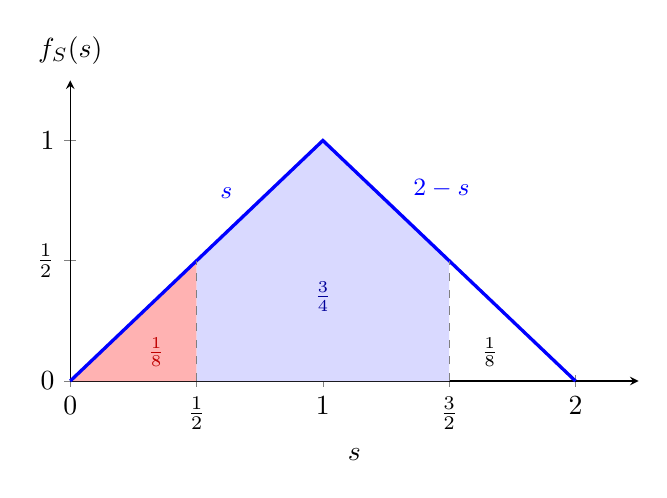
\begin{tikzpicture}
	\begin{axis}[
		axis lines=left, xmin=0, xmax=2.25, ymin=0, ymax=1.25,
		xtick={0,0.5,1,1.5,2}, xticklabels={$0$,$\tfrac12$,$1$,$\tfrac32$,$2$}, ytick={0,0.5,1}, yticklabels={$0$,$\tfrac12$,$1$},
		xlabel={$s$}, ylabel={$f_S(s)$}, ylabel style={rotate=-90, anchor=south, at={(axis description cs:0,1.02)}},
		width=8.8cm, height=5.4cm, clip=false
		]
		\addplot[fill=red!30, draw=none] coordinates {(0,0) (0.5,0.5) (0.5,0)} -- cycle;
		\addplot[fill=blue!15, draw=none] coordinates {(0.5,0) (0.5,0.5) (1,1) (1.5,0.5) (1.5,0)} -- cycle;
		\addplot[blue, very thick] coordinates {(0,0) (1,1) (2,0)};
		\draw[gray, dashed] (axis cs:0.5,0) -- (axis cs:0.5,0.5);
		\draw[gray, dashed] (axis cs:1.5,0) -- (axis cs:1.5,0.5);
		\node[red!75!black, font=\small] at (axis cs:0.34,0.12) {$\tfrac18$};
		\node[blue!60!black, font=\small] at (axis cs:1,0.35) {$\tfrac34$};
		\node[font=\small] at (axis cs:1.66,0.12) {$\tfrac18$};
		\node[blue, anchor=south east, font=\small] at (axis cs:0.68,0.72) {$s$};
		\node[blue, anchor=south west, font=\small] at (axis cs:1.32,0.72) {$2-s$};
	\end{axis}
	
\end{tikzpicture}
\end{document}
